\documentclass{article}
\usepackage{amsmath}
\usepackage{amsfonts}
\usepackage{amssymb}
\usepackage{courier}
\usepackage{graphicx}
\usepackage{subfig}
\usepackage{listings}
\usepackage[margin=1in]{geometry}

\begin{document}
\nocite{*}

\tableofcontents

\newpage

\listoffigures

\newpage

\begin {abstract}
In recent years, the City College of New York has seen its Computer Science program grow immensely, to the point of overcrowding. This has negative implications for both students and professors, particularly in introductory computer science courses in which constant feedback, iteration and collaboration with others is key to success. In this paper we propose various models for collaboration amongst students in all course levels using distributed version control systems and implement a secure and efficient tool\footnote{Technetium: https://technetium-redux.herokuapp.com/} for visualizing collaborative efforts by observing past work [5]. Lastly, we lay the foundation for future work around additional collaborative metrics, features and plagiarism detection.

\end {abstract}

\section {Introduction}

With an increased popularity in the computer science major in recent years, overcrowding in introductory computer science lectures has become rampant. At City College in particular, classes are overflowing with nearly a 100 students per 1-2 professors, preventing professors from providing the necessary attention their students need at this particularly early stage in their programming career. On the other hand, in the current generation of software engineering, learning how to use Version Control Systems (VCS) has become an absolute and necessary skill  for all students studying computer science to learn. With these two points in mind, how can we leverage VCS to help alleviate the problem of providing feedback to students while at the same time teaching students how to successfully collaborate together? We will explore both of these ideas in this paper and provide a technical solution to address these problems.

\subsection {Version Control Systems}

In Software Engineering, we are faced with one common problem - how does a group of individuals successfully collaborate on a project while sharing one codebase? Using a VCS, we can achieve precisely that. Currently, there are two well-known VCS: \emph{git}\footnote{Git: https://git-scm.com/} and \emph{mercurial}\footnote{Mercurial: https://www.mercurial-scm.org/}. These tools allow developers to collaborate on a group of files in a \textbf{project} while solving problems such as \textbf{communication} and \textbf{merge conflicts} between files. These projects are stored as \textbf{repositories} in the \textbf{cloud} through the use of \textbf{collaborative platforms} which are \emph{Github}\footnote{Github: https://github.com/} and \emph{Bitbucket}\footnote{Bitbucket: https://bitbucket.org/}. These platforms provide a service which allows developers to communicate, collaborate and control their codebase history. In this paper we will focus exclusively on using git repositories on Bitbucket.

\subsection{Benefits of VCS}

One common thing that students tend to do when working on software projects is to collaborate with other students. This allows them to learn from each other while at the same time having someone to bounce ideas off of in hopes of being able to solve their own problems. Since students already collaborate verbally with each other in class, one idea to handling overcrowding in classes would be to group students together. By having closely knit groups, students can learn from one another while at the same time being able to finish their numerous programming assignments. 

As beneficial as VCS are, they are often neglected throughout the computer science curriculum. While they are often viewed as tools for software engineering in the real world, they have numerous benefits to students and professors alike. VCS allow professors to proportionally determine the adversity that groups are experiencing as shown in [1], [3], [4] and even enhance spatial capabilities of young children [2]. In the upcoming sections we explore the features of VCS and the Bitbucket platform that students can use to their advantage.

\subsection{Version Control}

The keywords in VCS are \textbf{version control}, which in this context means to have the ability to have \textbf{multiple versions} of an existing codebase. Suppose that a student is working on a programming assignment and continuously \textbf{commits} code into the repository, but at a certain point checks in code which breaks existing tests in the assignment. Through the power of \emph{git}, the student can simply \textbf{roll back} their codebase to a previous commit at which everything was functioning properly. 

The power of version control really shines in group projects, as students will regularly break existing code. Even if students commit code which breaks the entire codebase, it can be reverted back to a previous commit in which everything was working fine. Moreover, students can directly place comments at any line of code in the codebase if they have questions about how something works. By adopting this approach, students are able to learn more in-depth from one another as opposed to just grabbing code from elsewhere without properly dissecting it.

\begin{figure}[h!]
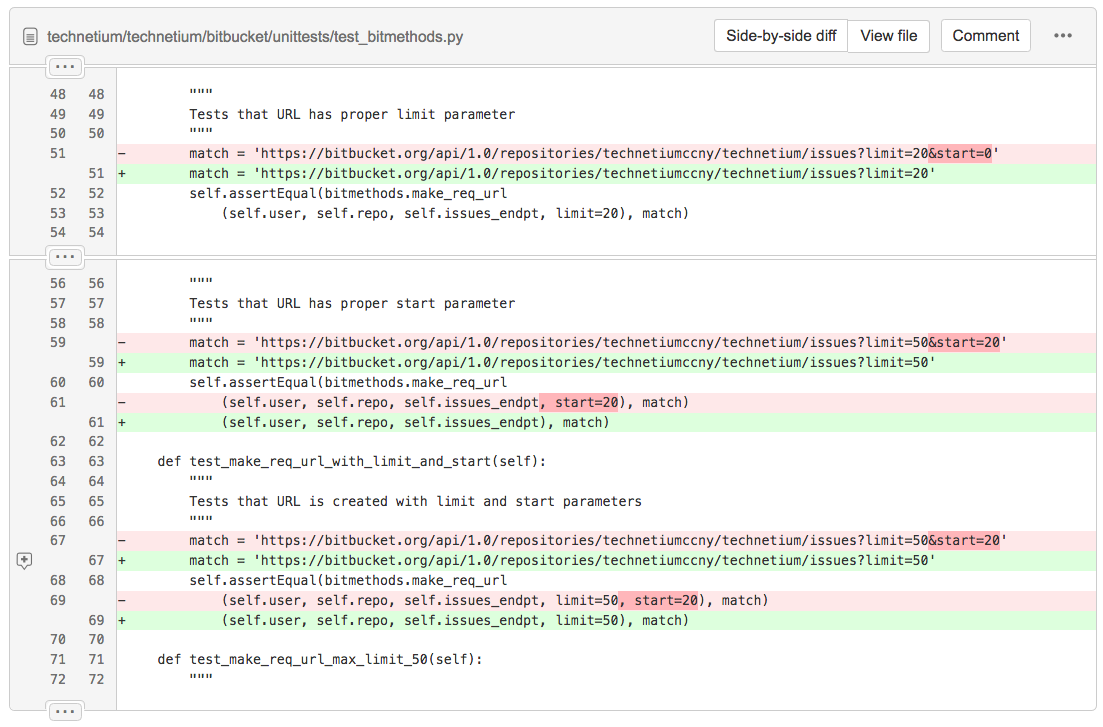
\includegraphics[height=10cm, width=16cm]{commit}
\caption{A sample commit}
\centering
\end{figure}

\subsection{Issue Tracking}

Bitbucket features a rich \textbf{issue tracker}, which allows individuals to create tickets detailing any bugs or features that need to be added to a project. The issue tracker can be utilized by creating a separate ticket for each feature that needs to be implemented in a given project:

\begin{figure}[h!]
\centering
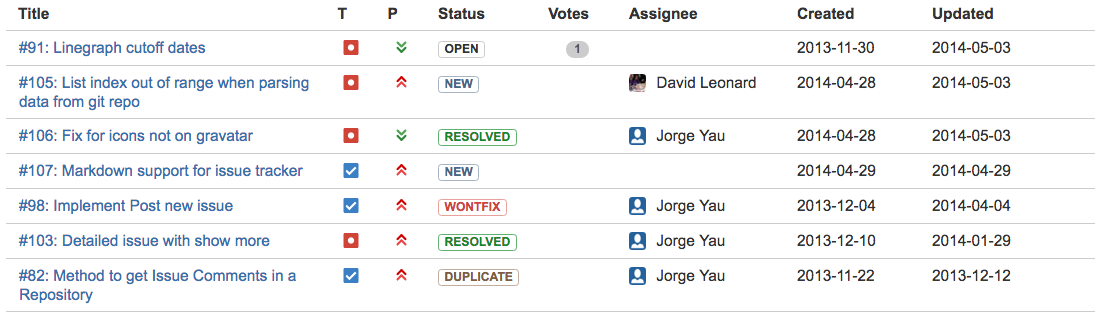
\includegraphics[height=4cm, width=14cm]{tracker}
\caption{Issues correlating to Project Features}
\end{figure}

As seen in Figure 2, additional labels may be added to an issue which show the status of the issue as well as the priority and assignee. By creating issues for all required features and distributing them amongst all group members, students can effectively split up a project in such a way that they can pick and choose which features they are comfortable with implementing. This approach helps to build the confidence in a student and ideally allows them to understand how other pieces of the program come together to form one coherent application. Additionally, issues may be closed directly by referencing them through commit messages:

\begin{figure}[h!]
\centering
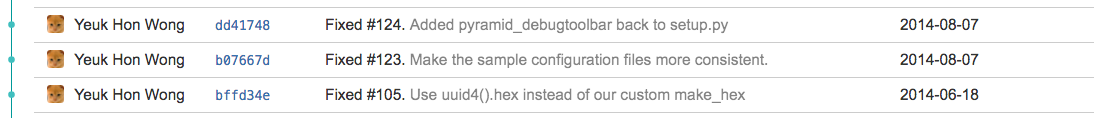
\includegraphics[height=2cm, width=14cm]{fix}
\caption{Resolving Issues directly through Commits}
\end{figure}

This promotes clean and real-world software engineering practices, while 
teaching students how to effectively maintain a real codebase on a smaller scale. Another approach to using issue trackers is to cycle issues around to other group members should an individual gets stuck with a particular feature - this is to help meet deadlines while also encouraging students to not give up and instead try their hand on another aspect of the program.

\subsection {Best Practices}

Students of all levels learn in their own personal way, and no two ways of thinking will always be the same. This is apparent when asking a student to implement a function which sums up all numbers in an array - two different approaches might be to use a \emph{for} loop while another approach will use a \emph{while} loop. In this case, neither approach is wrong or right, it is up to the student to decide. But what happens when students are given functions to implement which are more sophisticated? A professor will notice that students differ in:

\begin{itemize}
	\item {\textbf{Indentation}}: Students may indent with 2 or 4 spaces, or in the \emph{worst} case, left-justify everything.
	\item {\textbf{Non-descriptive Variable Names}}: Students may not use variable names which are descriptive, hence leading to confusion in the future.
	\item {\textbf{Comments}}: Students may not comment their code, which will cause problems in the future when reviewing for exams.
\end{itemize}

When working alone, students often do not gain insight as to how they may improve their skills or write readable code - a skill that has direct consequences when pursuing a career in software engineering. The best known way to remedy this is to read the source code of others, whether it be online, through peers or to read various programming books. In this model, students collaborating using VCS can observe how their peers write their own code and learn the best practices which work for them and overall get exposed to different ways of thinking.

\section {Project Types}

With the benefits of VCS covered, we now need to explore how students should appropriately create issue tickets for each feature which is needed in a given programming assignment. To do this, we explore various programming assignment formats.

\subsection {Project Skeletons}

A common format for giving students programming assignments is through the use of \textbf{project skeletons}, which consists of empty functions that are documented with comments regarding their implementations. In this scenario, it is trivial to create issues on Bitbucket for these assignments - every function which needs to be implemented will have a corresponding issue. To take things a step further, students can then assign these issues to themselves or other members in the group and add labels to functions which are blockers - meaning that their implementation is needed for other functions. In this sense, it allows students of all programming levels to effectively reason about their projects and to consider how to prioritize their implementation.

\subsection {Requirement Documents}

In higher level classes, sample code through project skeletons are often not given. In these situations, students are presented with documents which state the feature requirements that an application must satisfy. Despite this, it is not always clear what path a project should take when started. Should a base class be built first, or helper functions? By having an issue tracker, students are encouraged to sit down and properly think about the project and break it down into smaller, more manageable chunks. Moreover, students will gain deeper insight as to why \emph{feature x} should come before \emph{feature y} and in turn will have an easier time with their assignment. 

Overall, discussing projects at this granular level promotes a deeper understanding of what needs to be done. Often times students are thinking only about the end result and skip over the finer details, but this type of structured planning will save hours (if not days) of work. With the collaboration model fleshed out, we move onto our next problem - how can students properly be evaluated for any type of group project?

\section {Collaboration Evaluation}

The goal of collaboration is to have groups of students which effectively contribute to a group project. However, in a class full of students (and multiple sections), it becomes nearly impossible for a Professor to properly evaluate everyone fairly. In fact, it is hard enough to effectively determine if students have completed individual projects on their own. What about classes in which an individual's contributions to a group project determines their final grade? These are all difficult problems to solve in the classroom settings, however they become attainable through the use of version control. This brings us to the main focal point of the paper - implementing a tool which can effectively visualize contributions of individuals to a group project.

\subsection {Metrics}

As we have seen in Section 2, version control systems provide us with the ability to track issues and commits. However, we are not limited to these metrics alone - there are various other parameters which are readily made available to us:

\begin {itemize}
	\item {\textbf{Lines of Code}}: How many lines of code did each student contribute to the project? This can be attributed to how much work has gone into their implementations.
	\item {\textbf{Commit Comments}}: How many comments on individual commits did each student create? These can be attributed to a student's curiosity and willingness to understand the codebase.
	\item {\textbf{Issue Comments}}: How many comments on feature issues did each student make? These are attributed to meaningful discussion of features, links to helpful resources and suggestions from other members.
	\item {\textbf{Issues Closed}}: How many issues were closed by each student? These correlate to how many features were implemented by each individual student.
\end {itemize}

Individually, these parameters are not particularly useful nor do they properly demonstrate the performance of a student. However, putting them all together will paint a meaningful and convincing story regarding the lifespan of a project as well as allowing professors to understand how students are performing. We begin by describing the collection of these parameters for a given project. 

\subsection {Bitbucket API}

Gathering the data needed for a given project is too tedious to be done by hand, however Bitbucket provides an \textbf{Application Program Interface (API)} which allows us to programmatically query data for a given project. An API is simply a web server which understands HTTP requests and responds with data from it's database corresponding to the query parameters it has received. For example, the viewing the url https://api.bitbucket.org/2.0/repositories/DrkSephy/wombat/commits/master?page=1 in any browser will respond with data corresponding to the commits in the repository \emph{wombat} belonging to the user \emph{DrkSephy}. A subset of the output may be found below:

\begin{figure}[h!]
\centering
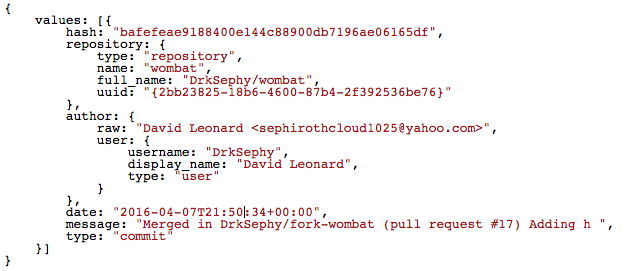
\includegraphics[height=6cm, width=14cm]{api}
\caption{Sample Data returned by Bitbucket API}
\end{figure}

Here, we can see various data regarding \emph{commits} in the repository named \emph{wombat}. Among this data, we can see every commit that has occurred along with the user who created the commit as well as the timestamp that it was created/updated. Using various other API endpoints, we can gather all of the necessary data to create an interactive visualization tool. However, we must discuss limitations of accessing data through the Bitbucket API.

\subsection {Privacy and Authentication}

A repository on Bitbucket may be set to \emph{public} (any user can view the contents of the repository), or \emph{private} in which nobody except the users given access to the repository may view its contents. Private repositories allow students to work in safety that no other individual can access their repository and view their code, preventing copying, cheating or other malicious intentions. However, accessing data from private repositories via the Bitbucket API requires a mechanism known as \textbf{\emph{authentication}}, in which an application goes through a protocol to access protected resources. Bitbucket relies on \textbf{OAuth 2.0}, which is a protocol for successfully authenticating a client application with Bitbucket's server for accessing protected resources. The following steps are required for gaining access to these resources:

\begin {enumerate}
	\item Create an OAuth consumer, which is our application in this case. 
	\item Using a given \textbf{secret key}, the consumer makes an HTTP request to get an authorization code.	
	\item Server (Bitbucket Server) issues an \textbf{Authorization Code}.
	\item Consumer redirects the user to Bitbucket's login page using the Authorization code.
	\item Resource owner (Bitbucket) grants access to the consumer (our application).
	\item Server accepts / rejects the user authorization.
	\item Consumer requests an \textbf{Access Token}.
	\item Server responds with the \textbf{Access Token}.
	\item Consumer can now access protected resources using this access token.
	\item The server responds with the protected resource.
\end {enumerate}

\begin{figure}[h!]
\centering
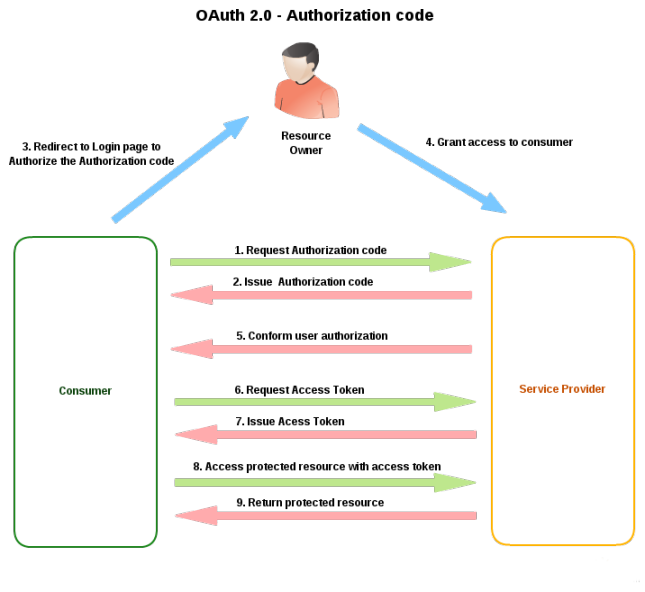
\includegraphics[height=13cm, width=14cm]{oauth}
\caption{OAuth 2.0 Protocol}
\end{figure}

At the end of this entire protocol, steps 9 and 10 repeat until the access token expires. Once an access token expires, the consumer must refresh their token by re-negotiating with the server to gain a new access token.

\section {Application Architecture}

An important decision in our project is to properly choose the tools that are needed to handle the tasks required. In this section we explain the problems and decisions that went into deciding our architecture, which can be seen in Figure 6.

\begin{figure}[h!]
\centering

\includegraphics[height=3cm, width=14cm]{arch}
\caption{Application Architecture}
\end{figure}

\newpage

The most important aspect of this project will be it's performance, both on the client-side and server-side. We begin by discussing performance of the client-side, with respect to rendering data to the client (web browser).

\subsection {React.js}

Given a class of 100 students with groups consisting of roughly 4$\sim$5 students, a Professor will have to visualize data for 20$\sim$25 projects. As such, we will find ourselves rendering various data components which need to be efficient over time. Rendering data on the web browser requires modifying the \textbf{Document Object Model (DOM)} tree, which represents the layout of a web page. 

\begin{figure}[h!]
\centering
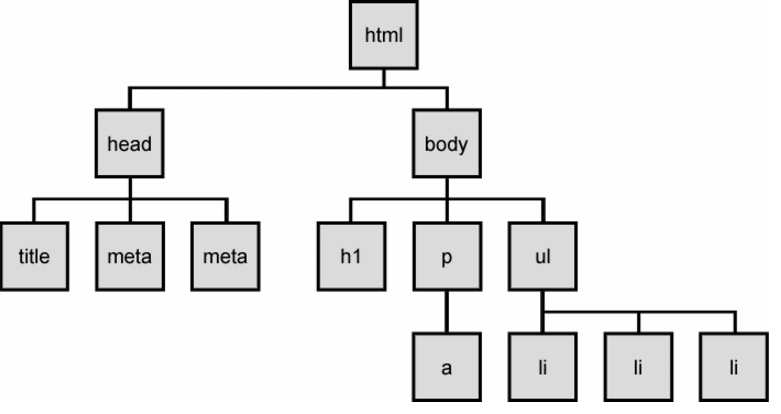
\includegraphics[height=8cm, width=14cm]{dom}
\caption{Document Object Model Tree}
\end{figure}

In terms of efficiency, updating the DOM tree consists of completely re-writing the tree from scratch. When updating the tree with new data and elements, this becomes costly in terms of node updates and rendering. Luckily, Facebook has released a cutting-edge library called \textbf{React} which is used for building sleek and efficient User Interfaces. React's power is it's ability to update the DOM tree in $\mathcal{O}(n)$ consistently through it's efficient diffing algorithm. Instead of thrashing the entire DOM tree and rebuilding it from scratch, React computes a shadow DOM which shows the change in nodes from the actual DOM, and uses this to update the actual DOM by replacing/removing any nodes which have been marked for update. While rebuilding the tree itself takes on average $\mathcal{O}(n)$, the known lower bounds are $\Omega (n^2)$ and the worst case is  $\mathcal{O}(n^3)$.

At a high level, React's reconciliation works by using hand-crafted heuristics which help to predict which parts of the DOM tree are more likely to be updated. Fundamentally, this problem is known as the \textbf{tree edit distance} problem [13], in which we want to compute the minimal-cost sequence of node edit operations to transform one tree into another. In our application, we will often find ourselves updating visualizations and datasets which will benefit from this efficient algorithm, which in turn will allow us to build a highly responsive user interface.

\begin{figure}[h!]
\centering
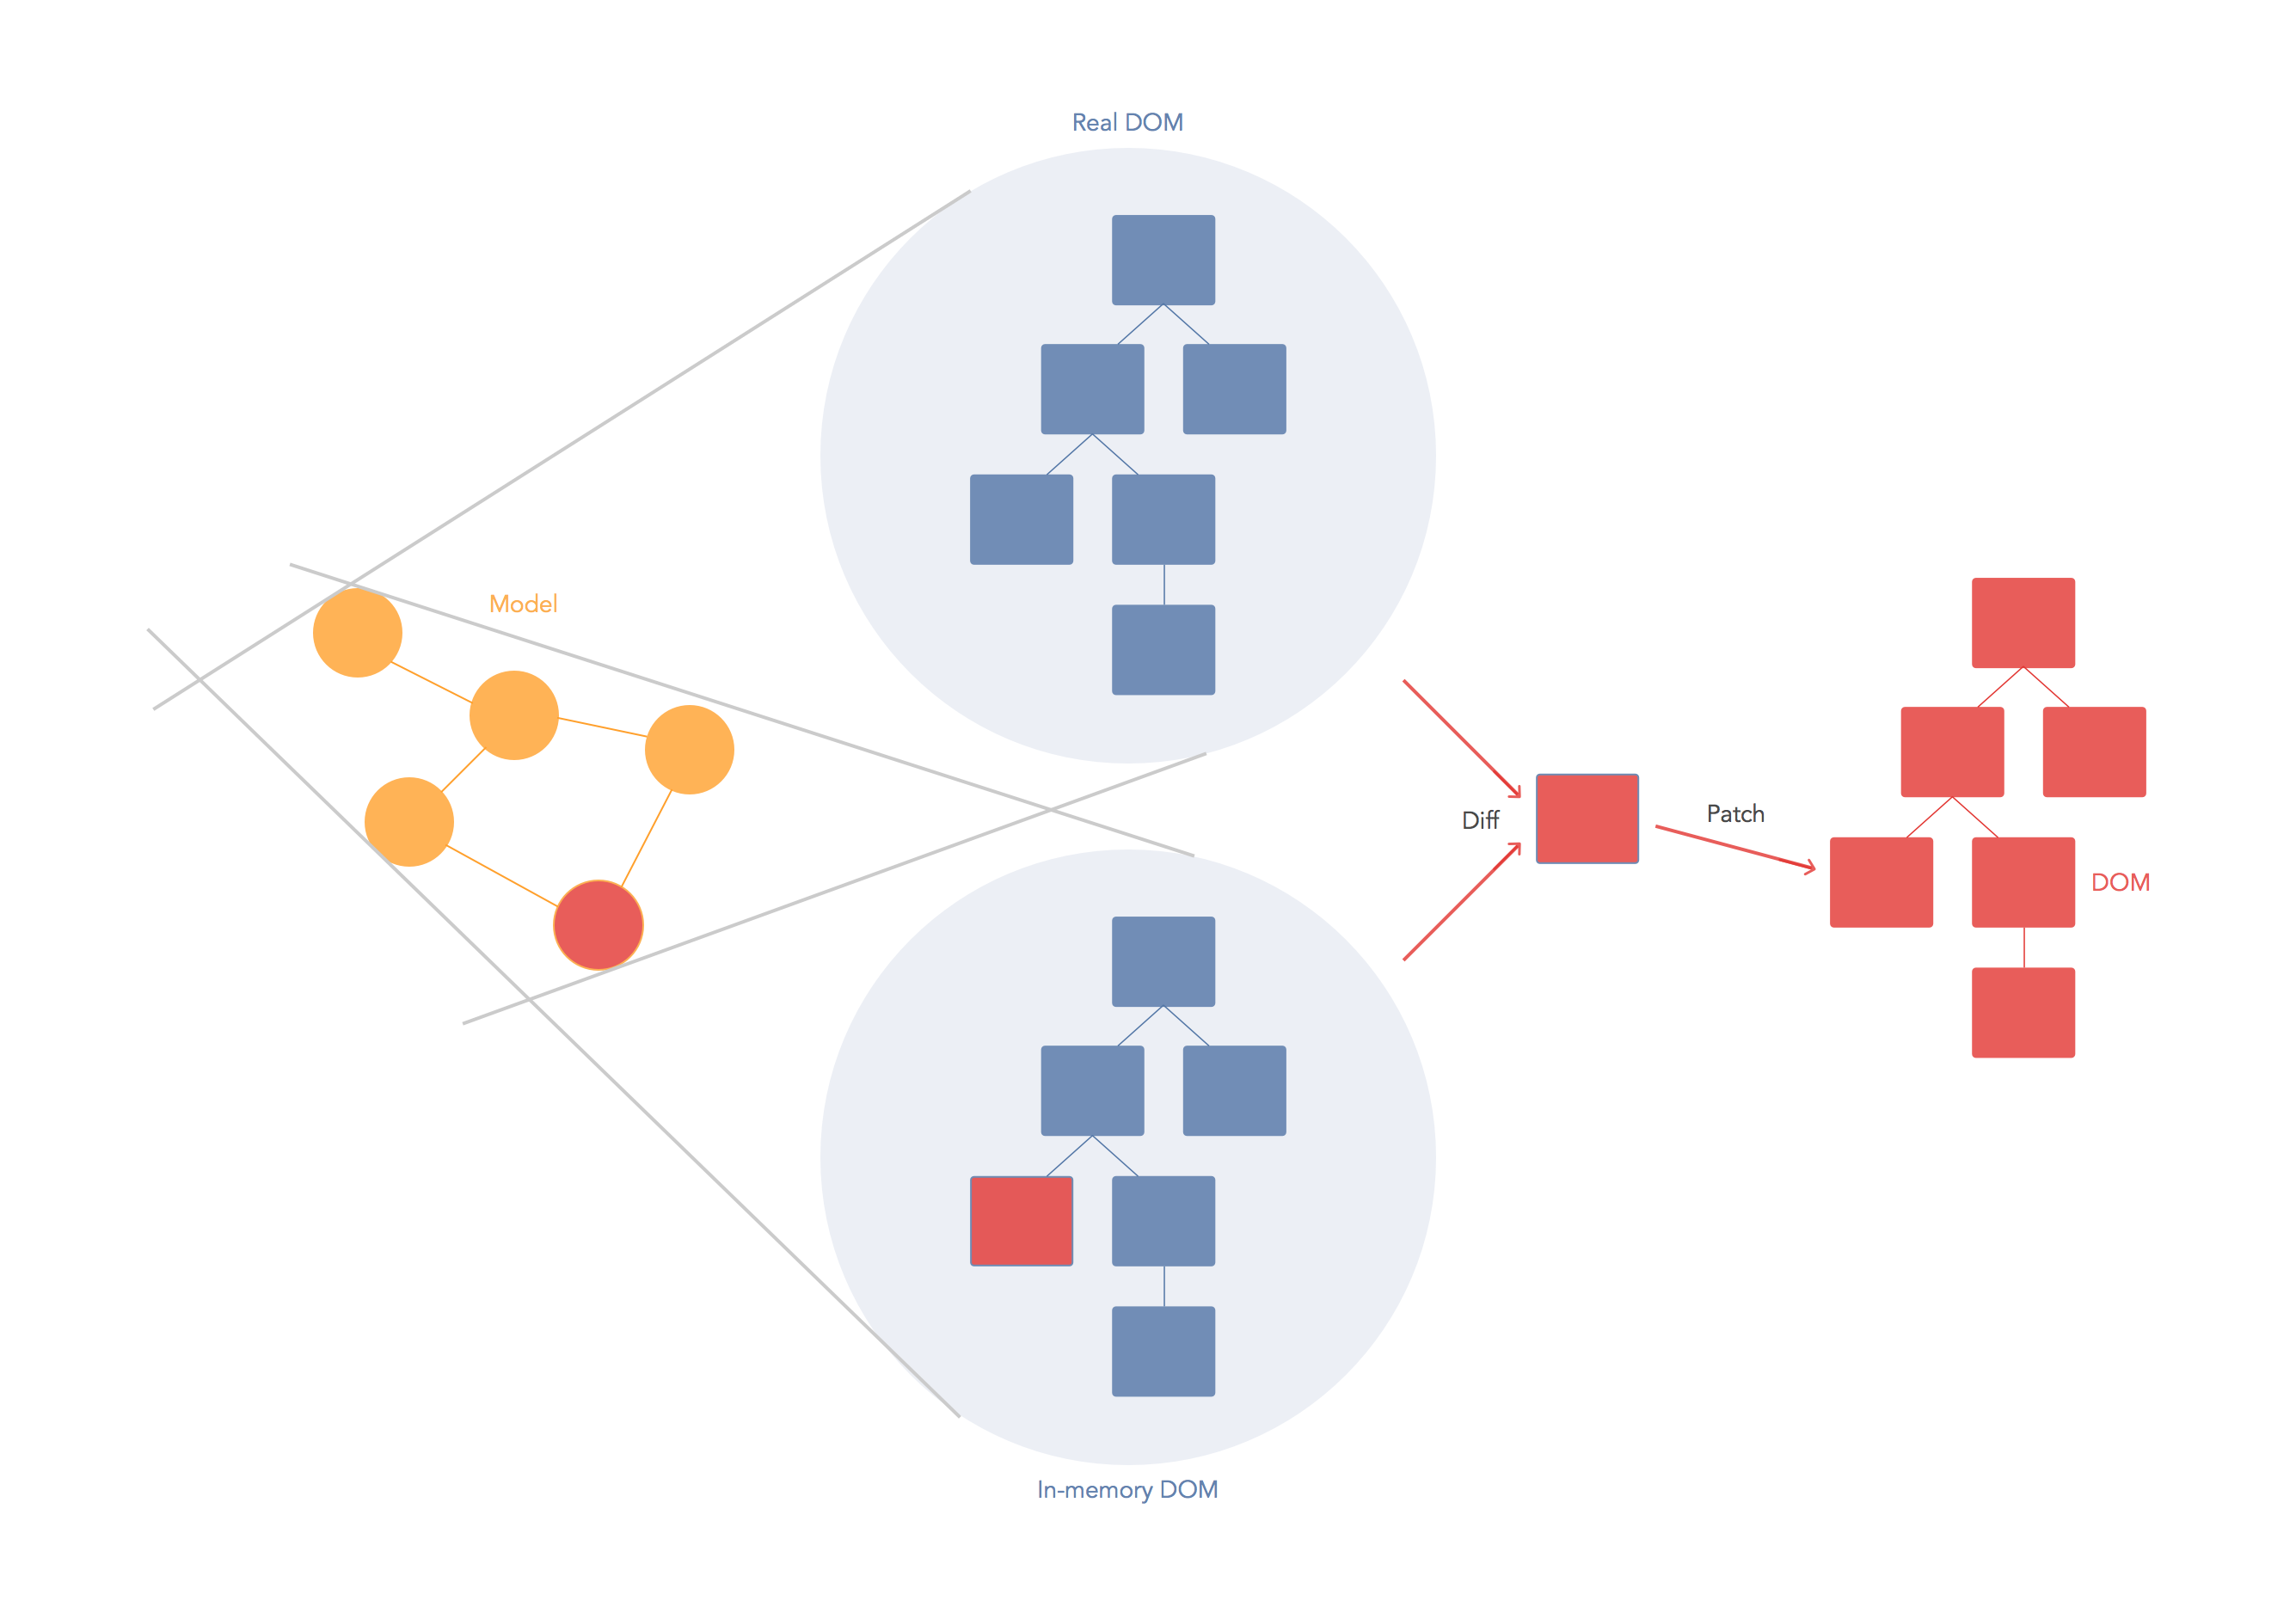
\includegraphics[height=11cm, width=14cm]{reconciliation}
\caption{Reconciliation of the Document Object Model Tree}
\end{figure}

\subsection {Node.js}

Now that our client-side technology stack has been decided, we move to our server-side. The server will have the following tasks:

\begin {itemize}
	\item {\textbf{Authentication Flow}}: The server will be needed for negotiating with Bitbucket to gain access tokens.	
	\item {\textbf{Re-negotiating Access Tokens}}: When a user's access token has expired, the server will need to automatically re-negotiate for an access token.
	\item \textbf{Fetching Resources}: The server will be responsible for fetching all data through queries on the client-side application.
	\item {\textbf{Communication with the database}}: Whenever new data arrives, the server will communicate with the database in order to store responses.
\end {itemize}

The server also needs to be able to handle \textbf{concurrent requests} without blocking the main execution thread. Hence, we choose \textbf{Node} - an efficient and well-tested server-side implementation written in JavaScript. In fact, Node is optimized to use the V8 runtime, which is the fastest JavaScript rendering engine. With these features, we can asynchronously handle hundreds of requests to Bitbucket's server in order to fetch all of the data needed for our application in parallel.

\subsubsection {Security Concerns}

As we previously mentioned, a server is needed for handling Authentication Flow and re-negotiating access tokens. The reason for this is that is has been shown that pure client-side authentication flows are vulnerable to various JavaScript attacks which can intercept and tamper with the request. Moreover, what does the client-side application do with the access token that is received after negotiating with the resource server? One solution is to store the token inside the browser through the use of a \textbf{cookie}, however this cookie is not secure and can be extracted using malicious JavaScript which in turn would lead to the application being compromised [7] [9]. 

In order to solve this problem, using a server to handle our negotiation will lead to our application being secure from these malicious attacks [10]. Lastly, we use the server to communicate with the database for storing user access tokens, as opposed to storing them on the client browser [11].

\subsubsection {Server-side Rendering}

One major benefit of the client-server relationship is our ability to render the HTML on the server and send it to the client. Through React's DOM \textbf{reconciliation}, if the client-side HTML does not match that of the server, it will automatically update the DOM to be synced with the server. Overall, this provides a massive performance gain in rendering the pages [6] of our application and prevent the client from corrupt HTML.

\subsection {Express.js}

In order to handle all of our API requests, we use \textbf{Express} which is an HTTP framework that is built on top of Node. This will allow us to send concurrent HTTP requests to the Bitbucket API which in turn will respond with the data we need to process. Express allows us to define simple HTTP routes, some of which are shown below:
\newline 

\begin{lstlisting}[frame=single]
app.get('/api/count', isAuthenticated, (req, res) => {
  getJSON('resource_url', req.user.authToken)
  .then((data) => {
    res.send(data);
  });
});
\end{lstlisting}

\vspace{0.5cm} 

\begin{lstlisting}[frame=single]
/**
 * GET /api/subscriptions
 * Returns the users subscriptions.
*/
app.get('/api/subscriptions', isAuthenticated, (req, res, next) => {
  User.findOne({ username: req.user.username }, (err, user) => {
    if (err) return next(err);

    if (user) {
      res.send(user.subscriptions);
    } else {
      res.send([]);
    }
  });
});
\end{lstlisting}

\newpage

\subsection {MongoDB}

The last component of our architecture is the database. In this application, we are primarily dealing with \textbf{JavaScript Object Notation (JSON)} - a lightweight response format returned from HTTP requests. Our data flow consists of the client-side application sending queries to the server, which in turn will respond with JSON data. This JSON is parsed and sent back to the client for rendering, and is also needs to be stored in the database for \textbf{caching} these web responses. JSON data consists of arbitrary key/value pairs, which makes it difficult to create schemas to store our data. As such, we use \textbf{MongoDB} - a document-based database which works very well with JSON data.

\subsubsection {Caching}

While the browser does a good job of caching repeated HTTP requests, we can speed up the turnaround from the client to the server and back by storing the parsed JSON on the server inside of the database. In this setup, whenever the client makes an HTTP request to the server, the server will first check if this data is already stored within the database - if not, the server queries the new data and updates the database and the client. Otherwise, the JSON is returned directly from the database and the client will update.

\subsection {Asynchronous JavaScript and XML}

When a user requests data from the server, we must perform these requests in a non-blocking way. In order to do this, we must first understand how web requests work.

\subsubsection {Traditional Page Refresh}

When a user clicks a link or navigates to a new url in their browser, the following actions take place:

\begin {enumerate}
	\item The webpage makes an HTTP request to the server.
	\item The server responds with the assets (HTML, CSS, JavaScript).
	\item When the client makes a new request, this process repeats.
\end {enumerate}

Due to this nature, the entire page is refreshed. This is known as a \textbf{Traditional Page Refresh}, which is shown in the figure below.

\begin{figure}[h!]
\centering
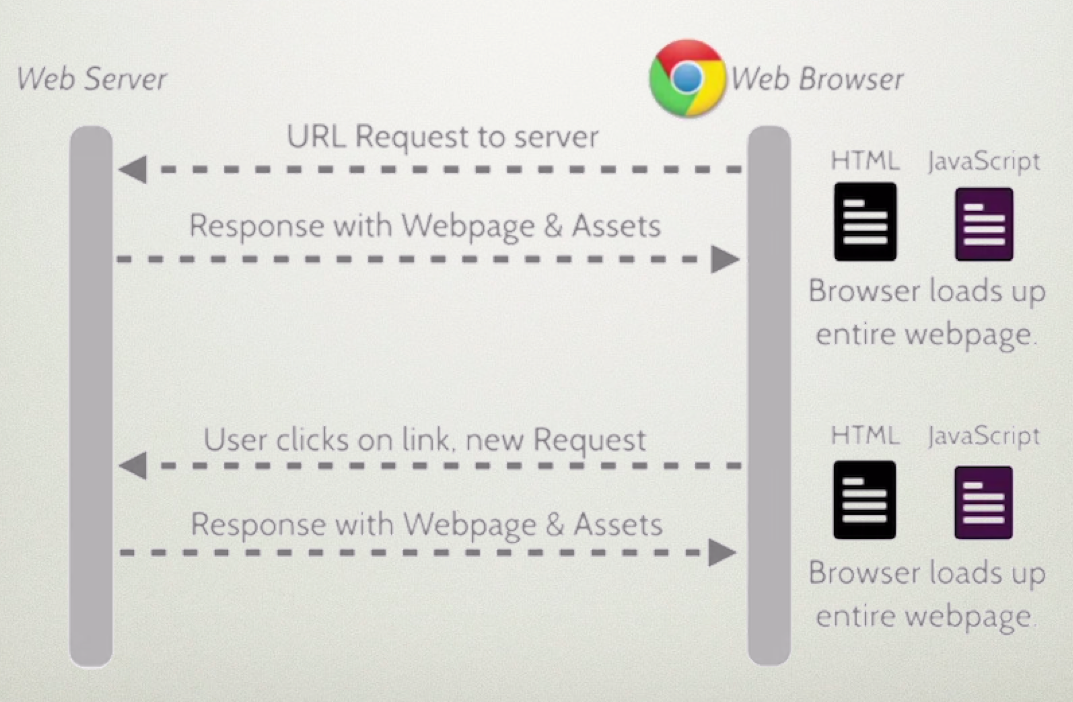
\includegraphics[height=7cm, width=14cm]{trad}
\caption{Traditional Page Refresh}
\end{figure}

\newpage

A more efficient way to update the contents of a web page is to use AJAX, which allows a client-side application to communicate with a server and receive data back in the format of JSON, XML, HTML and even text. In this new scheme, the following actions take place:

\begin {enumerate}
	\item The webpage makes an HTTP request to the server.
	\item The server responds with the assets (HTML, CSS, JavaScript).
	\item When the client makes a new request, the server will instead respond with JSON data, which is loaded into the existing page.
\end {enumerate}

By sending JSON back and forth between the server and the client, we create a seamless user experience which does not require page refreshes. This architecture is shown below:

\begin{figure}[h!]
\centering
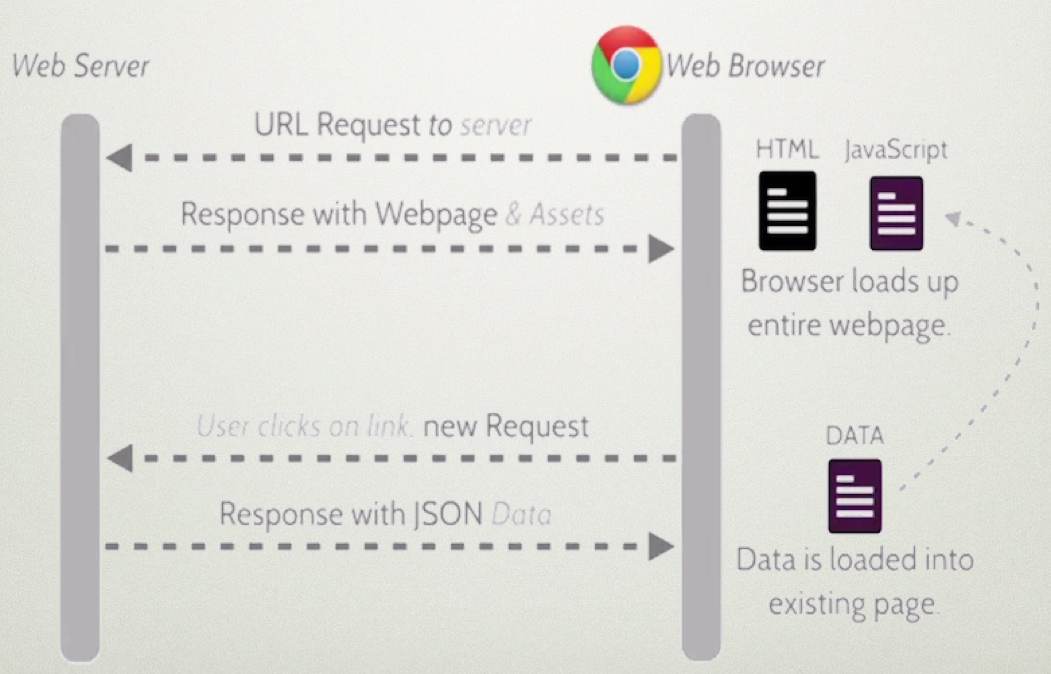
\includegraphics[height=7cm, width=14cm]{trad2}
\caption{Asynchronous JavaScript and XML refresh}
\end{figure}

\subsection {Architecture Summary}

As we have described, we have an efficient pipeline ranging from client-side DOM rendering to concurrent HTTP requests on the server tied together seamlessly using MongoDB - all operating on a lightweight response format (JSON) through a series of AJAX calls. In turn, we will be able to deliver a fast experience to the end-user which will consist of both Professors and Students. 

\section {Application Features}

With our architecture decided, we move onto describing all of the features of our application. The end goal of this application is to give the viewer a high level understanding of the level of progress in a project. We also want students to be able to get immediate feedback as to how they are performing in a group project.

\subsection {Authentication}

When the user loads the application, they need to be able to authenticate with Bitbucket easily with one click. As stated, this is needed so that they can access any private repositories which they own. In order to implement the OAuth 2.0 protocol on the sever, we use a package called \textbf{passport.js}, which securely implements this protocol and allows us to fetch access tokens [8]. Once the user is successfully authenticated with OAuth, they are redirected to the dashboard. 

\subsection {Subscription Manager}

In order to generate visualizations for a project, the user needs a way to specify which repository they would like to process. We create a subscription manager component which displays all of the repositories which the authenticated user has read access to, shown in Figure 11. 

\begin{figure}[h!]
\centering
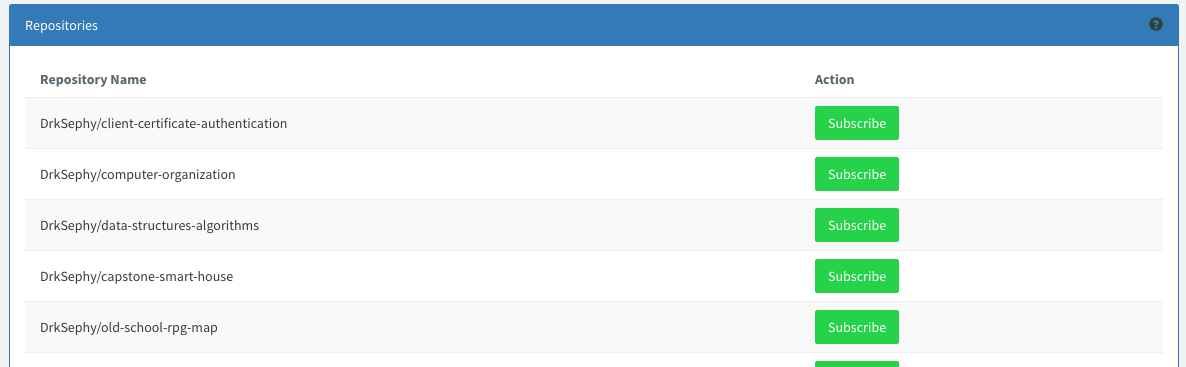
\includegraphics[height=6cm, width=17cm]{sub}
\caption{Subscription Manager}
\end{figure}

Here the user may quickly subscribe/unsubscribe to any of their repositories with the click of a button. While this is convenient for the user, it may be slow if they have many repositories to scroll through. To circumvent this, we have also created an alternative subscription manager shown in Figure 12 which allows the user to subscribe to a repository given a known repository name and Bitbucket username.

\begin{figure}[h!]
\centering
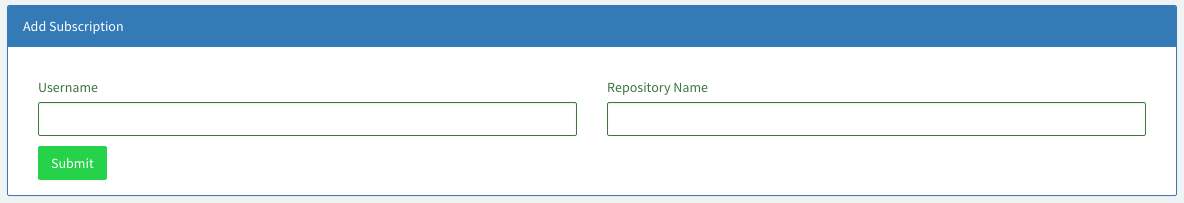
\includegraphics[height=3cm, width=17cm]{alt}
\caption{Alternate Subscription Manager}
\end{figure}

Once the user subscribes to a repository, the navigation bar will update with the list of subscribed repositories, shown in Figure 13.

\begin{figure}[h!]
\centering
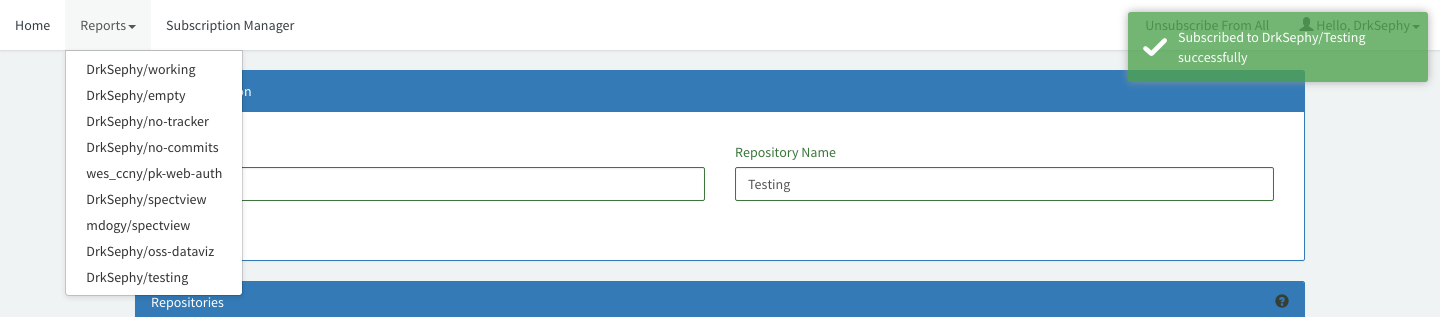
\includegraphics[height=4cm, width=17cm]{update}
\caption{Navigation Bar Updates}
\end{figure}

Clicking one of the items in the navigation bar will take the user into the visualization of the clicked repository name, which we discuss next.

\subsection {Repository Visualization}

The repository visualization consists of the following data components:

\begin {itemize}
	\item \textbf{Commits Card}: Displays the number of commits over a given time frame, along with a sparkling chart detailing the data trend.
	\item \textbf{Issues Opened}: Displays the number of issues opened over a given time frame, along with a sparkline chart detailing the data trend.
	\item \textbf{Issues Assigned}: Displays the number of issues assigned over a given time frame, along with a sparkline chart detailing the data trend.
	\item \textbf{Issues Closed}: Displays the number of issues closed over a given time frame, along with a sparkling chart detailing the data trend.
	\item \textbf{Repository Statistics}: Displays the totals of commits, issues opened/closed/assigned/comments and pull requests throughout the entire repository over the course of time.
	\item \textbf{Time Series}: Displays the commits over a one week for the given repository.
\end {itemize}

We break down their functionality over the course of the next sections.

\subsubsection {Data Cards}

The goal of the \textbf{commits}, \textbf{issues opened}, \textbf{issues closed} and the \textbf{issues assigned} cards is to give an overview of these datasets over a specified time.

\begin{figure}[h!]
\centering
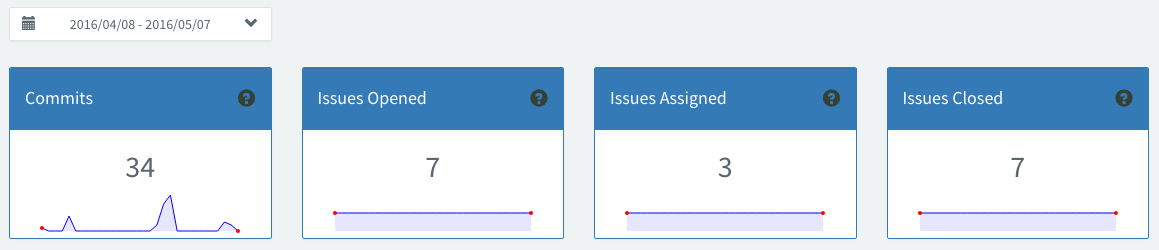
\includegraphics[height=4cm, width=17cm]{cards}
\caption{Data Cards}
\end{figure}

These parameters show arguably the most telling stories of the given repositories. Commits show that the repository is active, while the number of issues opened, assigned and closed demonstrate that features are being thought up and implemented throughout the given time frame. This data is further visualized through the underlying \textbf{sparkling charts}, which show how these data points are distributed over the time period. Moreover, users can use the date range picker in the top left to specify a time range to visualize new data as shown in Figure 14. Here, the user may pick from various preset date ranges such as \textbf{Last 7 Days}, \textbf{Last 30 Days} and \textbf{Last Month}.

\newpage

\begin{figure}[h!]
\centering
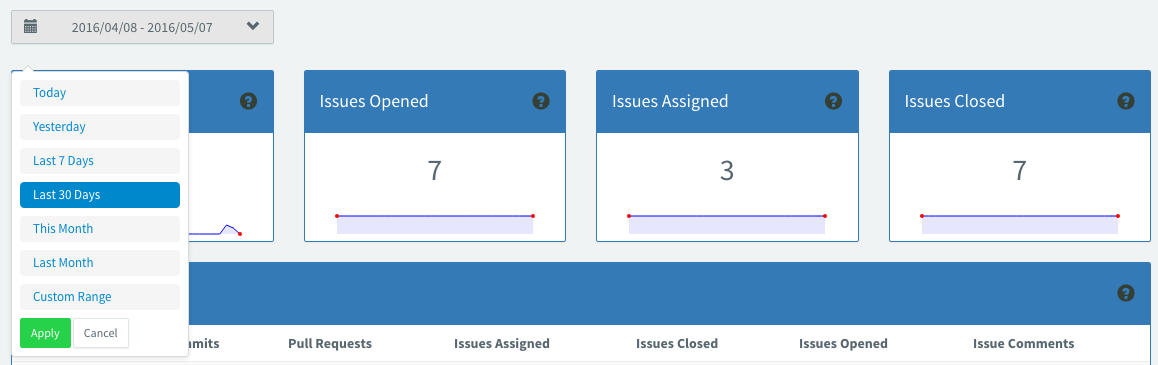
\includegraphics[height=5cm, width=17cm]{drop}
\caption{Date Range Picker}
\end{figure}

\vspace{0.5cm} 

Alternatively, the user may choose a custom date range as shown in Figure 15. This allows complete flexibility when selecting which data to visualize, even allowing the user to back to the beginning of time for a given project.

\vspace{0.5cm} 

\begin{figure}[h!]
\centering
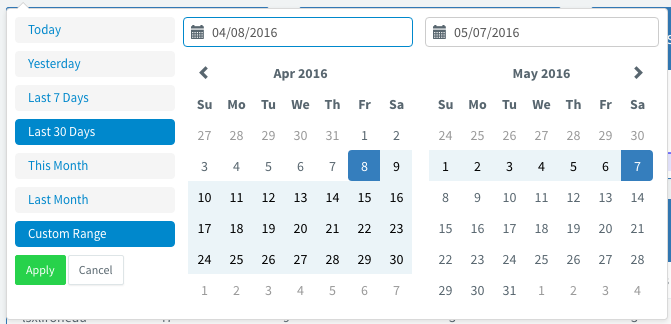
\includegraphics[height=8cm, width=17cm]{expand}
\caption{Expanded Date Range Picker}
\end{figure}

\subsubsection {Commit Time Series}

The last major component of our application is the \textbf{Commit Time Series}, shown in Figure 17. This allows students to see the commit history on a line plot over the last week. Currently, this feature is not tied to the custom date range picker but is planned in future work. At a glance, the time series allows both students and professors to quickly see the work that has been done in the given project.

\begin{figure}[h!]
\centering
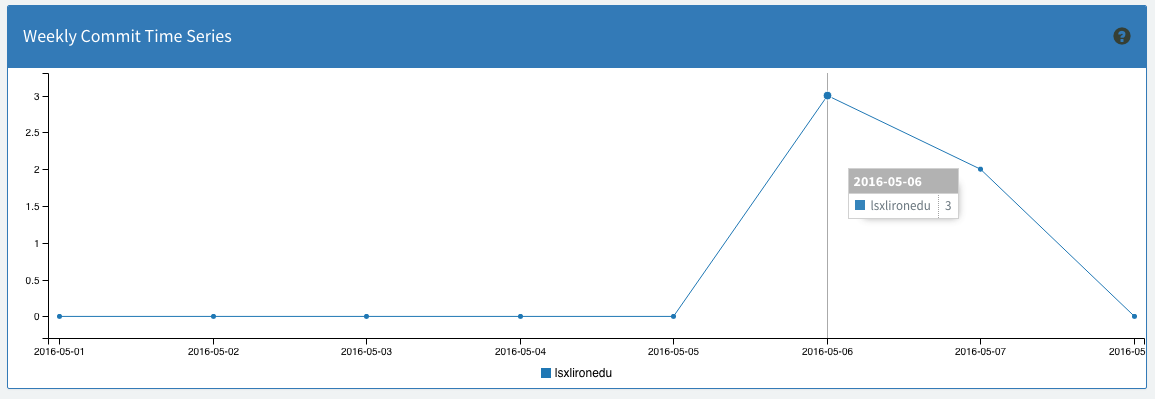
\includegraphics[height=5cm, width=17cm]{timeseries}
\caption{Weekly Commit Time Series}
\end{figure}

\section {Future Work}

While there are several key features in place, there still remains several features that we would like to implement. We review these features here.

\subsection {Plagiarism Detection using Graph Isomorphism}

Given two graphs $G_1$ and $G_2$ which contain the same number of vertices connected in the same manner are considered to be \textbf{isomorphic} to each other. More formally, two graphs $G$ and $H$ and a set of vertices $V_n = \{1, 2, ..., n\}$ are said to be isomorphic to each other if there exists a permutation $p$ of $V_n$ such that \{u, v\} is in the set of edges $E(G)$ $\iff$ $ \{p(u), p(v)\} $ is in the set of edges $E(H)$. 

\begin{figure}[h!]
\centering
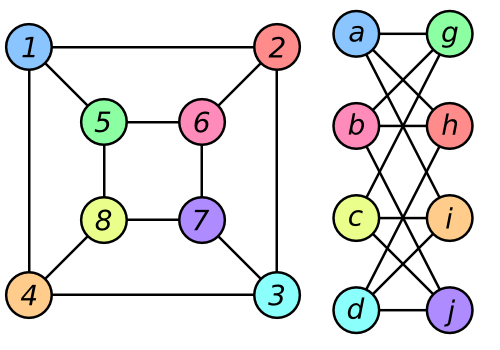
\includegraphics[height=5cm, width=8cm]{isomorphic}
\caption{Graph Isomorphism Example}
\end{figure}

Translating this notion to analyzing source code, it is possible to represent control flow of a program in terms of a graph. In this case, each \emph{function} would correspond to a node in the graph, and the transitions (\emph{edges}) would map to how these functions are transitioned to from the main program. Given two side-by-side programs, we can detect if these two programs are simply \emph{permutations} of each other - meaning that they are essentially replicated copies with functions swapped. This feature can be implemented in quasi-polynomal time [14] and there exist several heuristics for determining whether random graphs [15] and trees [16] are isomorphic. This feature is useful for detecting plagiarism between open-ended projects as described in Section 2.2, but doesn't hold up in assignments in which project skeletons are used.
\subsection {Cyclomatic Complexity}

In the case of project skeletons, we can employ the use of cyclomatic complexity which is a measure of program complexity by computing the number of linearly independent paths in the source code. Similar to Graph Isomorphism, we can construct a graph with nodes corresponding to \emph{functions}, \emph{modules}, \emph{methods} or \emph{classes}. We connect these nodes based on the progression of the program, i.e: some function \emph{x} calls function \emph{y}, and so on - known as the \textbf{control flow graph}. Using this metric, a professor can quickly tell if programs written by students have the same measures, thereby correlating the majority of students who are on the right track towards finishing the assignment.

\subsection {Exporting Visualizations as Reports}

The ability to export project visualizations as PDFs would be a useful feature for students to quickly summarize their weekly progress. Unfortunately, the complexity of writing a custom web scraper for applications whose data is updated dynamically using JavaScript is non-trivial and a project on its own, but can be implemented using tools such as PhantomJS \footnote{Headless WebKit JavaScript API: http://phantomjs.org/}.

\subsection {Lines of Code per Contributor}

While the number of lines of code written by each individual in a project is not a testament to participation, honesty or worthy of being graded, it is a useful metric to track. The feature for gathering this information has been implemented in this project, but was forced to be temporarily removed due to the excess amount of HTTP requests needed to be performed. For each commit, an additional request must be made to gather the lines added/removed which can easily add up to hundreds of commits for large projects. Due to the asynchronous nature of batching HTTP requests with JavaScript, sending this many requests to Bitbucket's server will prompt it to consider our application a bot and therefore would throttle our requests. In order to circumvent this, a rate limiter must be implemented which will carefully batch our requests into sizable amounts within a queue and send them out periodically.

\subsection {Support for Mercurial}

As mentioned earlier, Technetium only supports visualizing \emph{git} repositories on Bitbucket. Due to the difference in response formats between \emph{git} and \emph{mercurial} repositories, an entirely new set of API requests must be written to successfully visualize both types of version controlled repositories. While the underlying API on the server is a decent starting point, it would take considerable time to extend the application to seamlessly support both version control clients.

\section {Conclusion}

Throughout the course of this thesis, we have addressed the current problems that are being faced by both students and professors in introductory computer science courses (as well as higher level courses). To solve this, we have proposed two models with which assignments may be given along with encouraging group work. In order to promote feedback on productivity among both parties, we have implemented a working application which will allow the user to gain deep insights as to how students are performing in their assignments. We have leveraged various web technologies and their advantages to ensure a quick, efficient and secure application through both the client and the server as well as the response formats of our database. Overall, we believe that all programming courses which utilize our tool will benefit in both productivity, fairness amongst grading and shortening the feedback loop between professor and student.

As a graduate student at the City College of New York who has taken various programming courses, Technetium would have surely benefitted these classes by lightening the feedback load on professors while making fellow classmates aware of their performance in the class. Moreover, projects such as [12] can be used in conjunction with Technetium to not only provide collaborative visualizations, but to provide students programmatic feedback on their assignments through a distributed environment which runs test code against a student's code.

\newpage

\begin{thebibliography}{9}
 
\bibitem{einstein} 
Pekka M�kiaho, Timo Poranen, Ari Seppi
\textit{Version Control Usage in Students� Software Development Projects}.
International Conference on Computer Systems and Technologies - CompSysTech�14

\bibitem{einstein} 
Filipe Santos, Benjamim Fonseca, Leonel Morgado, Paulo Martins
\textit{A Version Control System as a Tool and Methodology to Foster Children�s Collaboration in Spatial Configuration Decision Tasks}.
Groupware: Design, Implementation, and Use, Volume 5411

\bibitem{einstein} 
Michael Cochez, Ville Isom�tt�nen, Ville Tirronen, Jonne Itkonen
\textit{How Do Computer Science Students Use Distributed Version Control Systems?}.
Information and Communication Technologies in Education, Research, and Industrial Applications, Volume 412

\bibitem{einstein} 
Michael Cochez, Ville Isom�ott�onen, Ville Tirronen and Jonne Itkonen
\textit{The Use of Distributed Version Control Systems in Advanced Programming Courses}.
ICTERI 2013

\bibitem{einstein} 
Louis Glassy
\textit{Using version control to observe student software development processes}.
Journal of Computing Sciences in Colleges, Volume 21 Issue 3, February 2006 

\bibitem{einstein} 
Madhukar N. Kedlaya, Behnam Robatmili, Ben Hardekopf
\textit{Server-Side Type Profiling for Optimizing Client-Side JavaScript Engines}.
DLS 2015 Proceedings of the 11th Symposium on Dynamic Languages

\bibitem{einstein} 
Vincent Delaunay
\textit{The concerning threat of Cross Sites Scripting (XSS) vulnerabilities}.
Dec. 2014

\bibitem{einstein} 
Ethan Shernan, Henry Carter,  Dave Tian, Patrick Traynor,  Kevin Butler
\textit{More Guidelines Than Rules: CSRF Vulnerabilities from Noncompliant OAuth 2.0 Implementations}.
Detection of Intrusions and Malware, and Vulnerability Assessment. Springer International Publishing, 2015. 239-260.

\bibitem{einstein} 
Kevin Fu, Emil Sit, Kendra Smith, Nick Feamster
\textit{Dos and Don�ts of Client Authentication on the Web}.
SSYM'01 Proceedings of the 10th conference on USENIX Security Symposium - Volume 10

\bibitem{einstein} 
Philippe De Ryck, Lieven Desmet, Frank Piessens, Wouter Joosen
\textit{Improving the Security of Session Management in Web Applications}.
(2013): 0-0.

\bibitem{einstein}
Andrew Bortz, Adam Barth, Alexei Czeskis
\textit{Origin Cookies: Session Integrity for Web Applications}.
Web 2.0 Security and Privacy (W2SP), 2011

\bibitem{latexcompanion} 
Michael D. Grossberg,  Joesan A. Gabaldon Jr., Paul K. Alabi, Jeremy K. Neiman, Irina Gladkova
\textit{Graphyte software for integrated remote sensing research using HPCC}. 
SPIE 2011

\bibitem{latexcompanion} 
Philip Bille
\textit{A Survey on Tree Edit Distance and Related Problems}. 
Theoretical Computer Science 337 (2005) 217 � 239

\bibitem{latexcompanion} 
Babai, L�szl�
\textit{Graph isomorphism in quasipolynomial time}. 
arXiv preprint arXiv:1512.03547 (2015)

\bibitem{latexcompanion} 
Czajka, Tomek, and Gopal Pandurangan
\textit{Improved random graph isomorphism}. 
Journal of Discrete Algorithms 6.1 (2008): 85-92.

\bibitem{latexcompanion} 
Buss, Samuel R.
\textit{Alogtime algorithms for tree isomorphism, comparison, and canonization}. 
Springer Berlin Heidelberg, 1997.

\end{thebibliography}

\end{document}
